\chapter{The CMS Detector}
\label{sec:cms}

The Compact Muon Solenoid (CMS) detector is one of two hermetic, general purpose detectors at the Large Hadron Collider.
The original motivation for the experiment was the discovery of the Higgs boson by observing its decays to photons, electrons, and muons.
Towards this end, the detector was built to fulfill the following goals:
\begin{itemize}
\item Unambiguous charge identification of muons with momenta up to 1\TeV
\item 1\GeV mass resolution on 100\GeV pairs of muons, electrons, and photons
\item Efficient triggering and tagging of $\tau$ lepton and $b$ quark decays
\item Good resolution on the hadronic energy and missing transverse energy
\item Sufficient time resolution to deal with 40 MHz of collisions
\end{itemize}
The CMS detector consists of four main subdetetors: the inner trackers, the electromagnetic calorimeter (ECAL), the hadronic calorimeter (HCAL), and the muon chambers.
The first three are within the field volume of the eponymous 3.8 T superconducting NbTi solenoid magnet while the muon chambers are embedded in the return yoke of the magnet.
Additionally, there is an online triggering system to reduce readout from 40 MHz to $\mathcal{O}(1)$ kHz for prompt reconstruction. 

\begin{figure}[htbp]
  \centering
  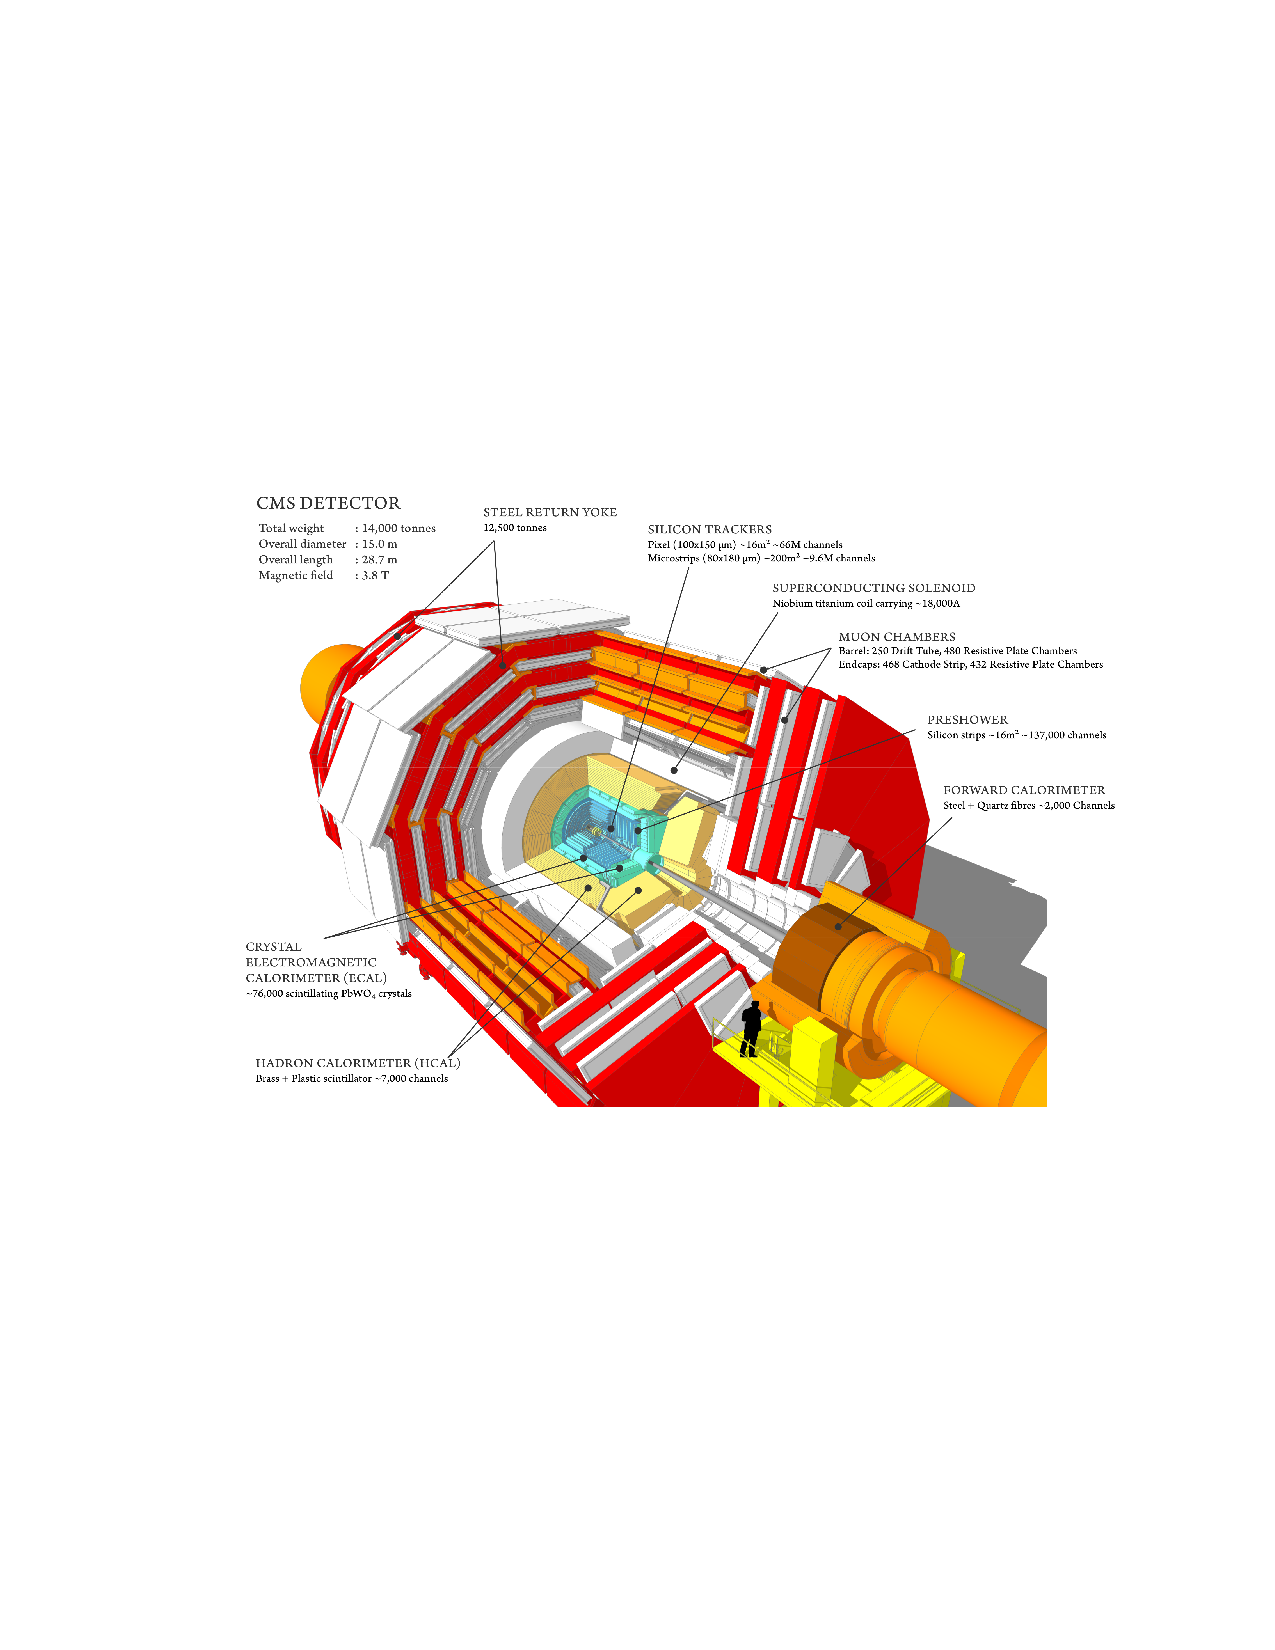
\includegraphics[width=0.9\textwidth]{Detector/Figures/cms_detector.pdf}
  \caption{
    A cutaway view of the CMS detector.
    The labels identify the solenoid as well as the different subdetectors and their components. 
    Reprinted from Reference~\cite{}. % http://cms.web.cern.ch/news/cms-detector-design
  }
  \label{fig:cms}
\end{figure}

The overall layout of the CMS detector is shown in Figure~\ref{fig:cms}. 
The CMS detector has a weight of 12500 tons, a length of 22 m, a diameter of 15 m, and a cylindrical geometry with concentric barrel shaped detectors in the central region and disc shaped detectors in the forward region.
The following coordinate system is used when working with the CMS detector:
\begin{itemize}
\item distance $z$ along the beam axis
  \begin{itemize}
  \item $z=0$ at the center of the detector
  \item positive corresponds to counter-clockwise as seen from the sky
  \end{itemize}
\item distance $r$ from the beam axis
\item polar angle $\theta$ measured with respects to the positive $z$-axis
\item azimuthal angle $\phi$ in the plane orthogonal to the beam axis
\end{itemize}
In addition to these four main coordinates, we define the right-handed cartesian $x$ and $y$ coordinates perpendicular to the beam axis, with the positive $x$-axis pointing from the center of the detector to the center of the LHC ring and the positive $y$-axis pointing upwards.

The four-momentum of a particle is $p = (p_x, p_y, p_z, E)$ in the cartesian basis 
%, where the first three components are space-like and the last one is time-like,
and a particle of mass $m$ produced at rest in the center of the detector has $p = (0, 0, 0, m)$.
While the momenta along the beam axis of the two incoming protons are equal, the momenta of the incoming partons involved in the hard scattering often are not as discussed in Section~\ref{sec:collider_pheno}.
Thus, we define two kinematic quantities that are Lorentz-invariant with respect to a boost along the beam axis:
the tranverse momentum $\ptvec = p_x \hat x + p_y \hat y$ with magnitude $\pt = \sqrt{p_x^2 + p_y^2}$ and the pseudorapidity $\eta = - \ln \tan\sfrac{\theta}{2}$.

In terms of \pt, $\eta$, and $\phi$, we have the following expressions for our cartesian variables: $p_x = \pt \cos \phi$, $p_y = \pt \sin \phi$, $p_z = \pt \sinh \eta$, and $E = \pt \cosh \eta$, with the last equality assuming the mass of the particle is negligible compared to its momentum.
In terms of our Lorentz-invariant coordinates, the four-momentum of a given particle is $p = (\pt, \eta, \phi, E)$. 
Additionally, the spatial separation of two particles is given by $\Delta R = \sqrt{(\Delta\phi)^2 + (\Delta\eta)^2}$ and the fiducial acceptance of the CMS detector is from $0 \le \phi < 2\pi$ and $-5 \le \eta \le 5$.

\section{Inner Trackers}
\label{sec:cms_tracker}

Closest to the interaction point, the inner trackers identify charged particles and measures their momenta.
Additionally, high resolution tracks are used to identify primary and secondary vertices.
The magnetic field in the tracker volume is uniform with strength 3.8 T and field lines parallel to the beam direction. 
The tracker volume extends to 1.2 m in $r$ and 2.9 m in $z$, providing coverage for $\abs\eta < 2.5$,  and is instrumented with silicon pixels and strips.
Each silicon sensor is a $p$-$n$ semiconductor junction with a bias voltage applied.
When a charged particle passes through the depletion region of the junction, electron-hole pairs are produced and collected by the readout electronics.
A schematic of the inner tracker system is shown in Figure~\ref{fig:cms_tracker}.

\begin{figure}[htbp]
  \centering
  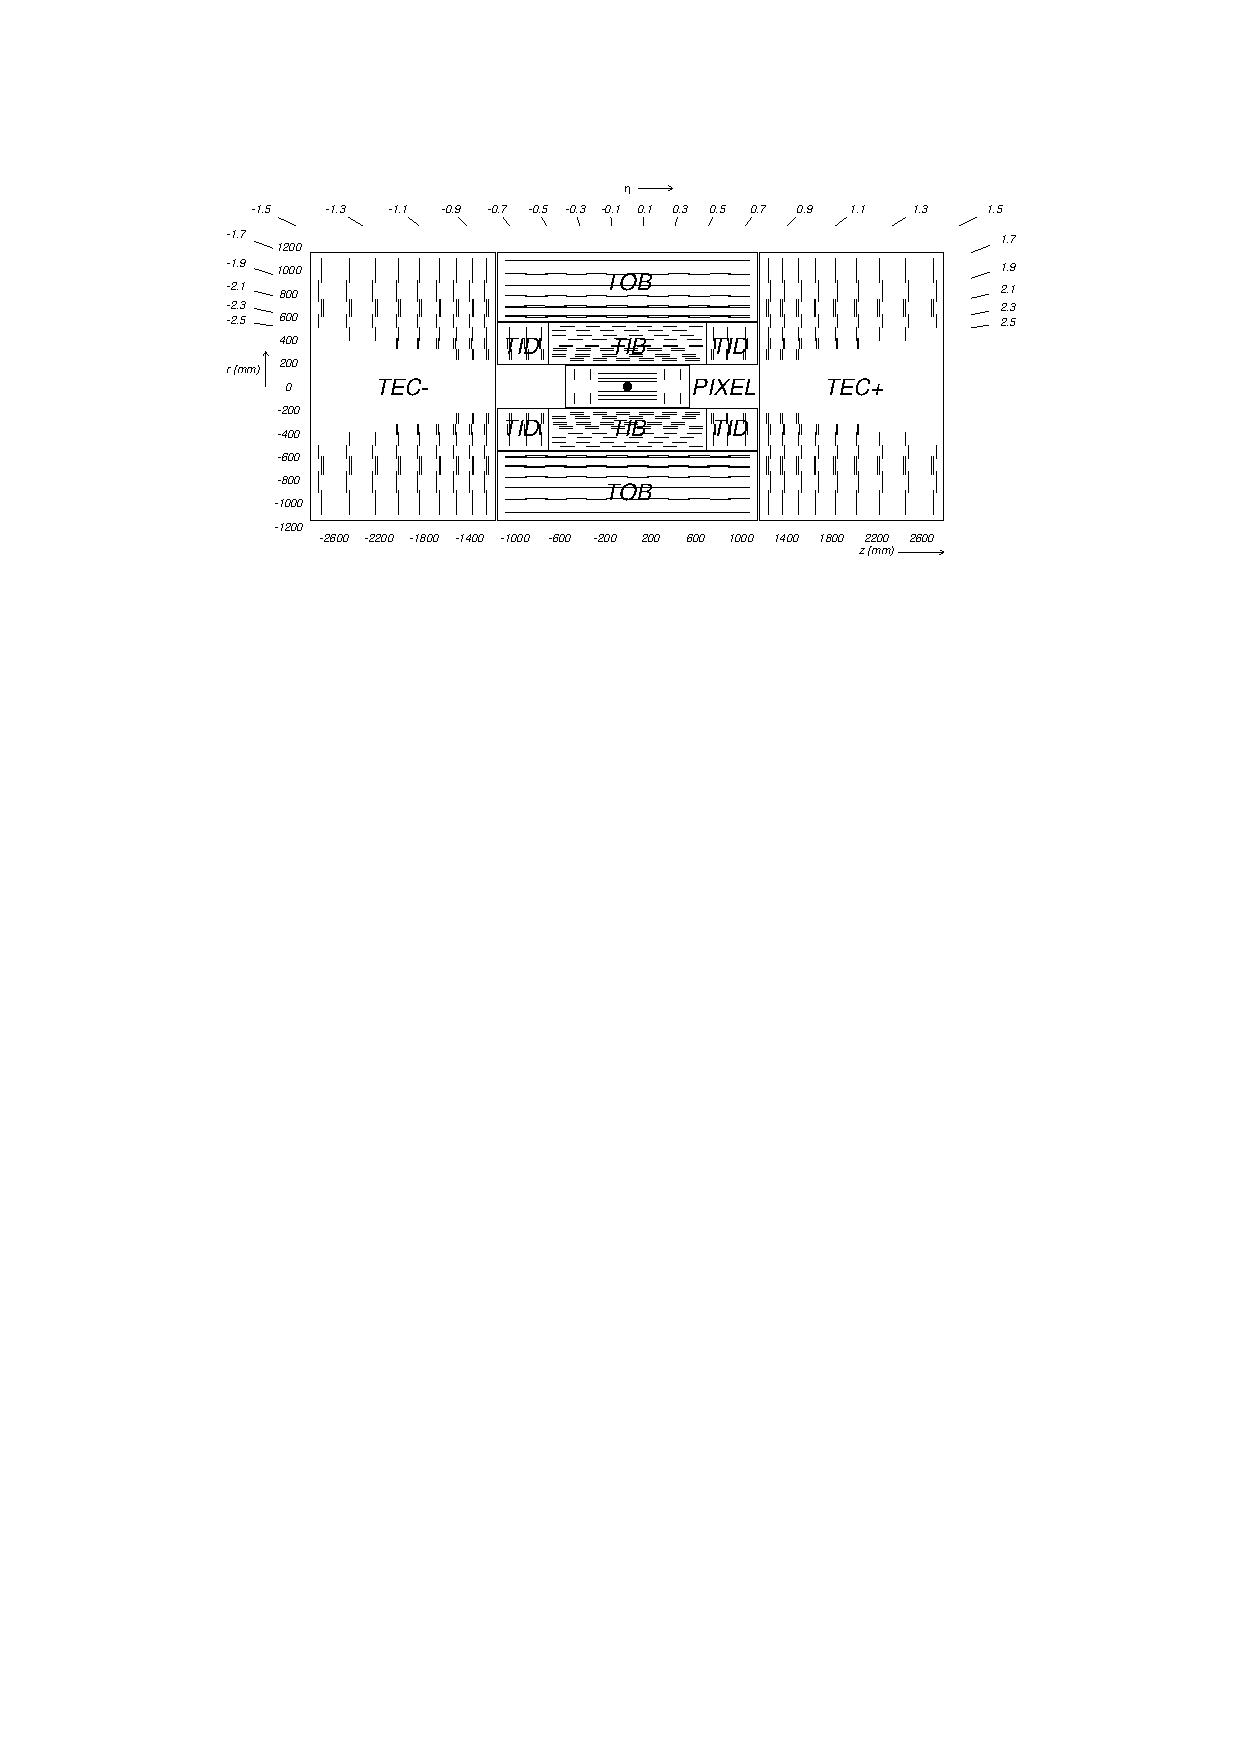
\includegraphics[width=\textwidth]{Detector/Figures/cms_tracker.pdf}
  \caption{
    A schematic view of the CMS inner tracker system.
    Silicon pixel and strip detectors are shown.
    The volumes labeled TIB, TID, TOB, and TEC are all strip trackers.
    The double lines indicate back-to-back modules that deliver stereo hits.
    % TIB = Tracker Inner Barrel, TID = Tracker Inner Disk, TOB = Tracker Outer Barrel, TEC = Tracker Endcap. 
    Reprinted from Reference~\cite{}. % https://iopscience.iop.org/article/10.1088/1748-0221/3/08/S08004/meta
  }
  \label{fig:cms_tracker}
\end{figure}

The 66 million individual pixel sensors, each measuring $285\mum\times 100\mum\times 150\mum$ in $r\times r\phi \times z$, are arranged into seven layers: three cylindrical barrels at $r = 4.4, 7.3, 10.2\cm$ and two bi-layer endcap annulli at $z = \pm34.5, \pm46.5 \cm$.
Due to the geometry of the pixel detector, tracks typically cross the sensor at a 20$^\circ$ angle, leading to the charge deposit from a single track to be shared among multiple pixels in the same layer.
The exact position of a particle in each layer is determined by interpolating the signals from multiple adjacent pixels with an analog pulse height greater than a tuneable read-out threshold.
Thus, each pixel hit is localized to an area of $\sim 15 \mum\times 20\mum$ in $r\phi \times z$, providing a much higher spacial resolution than the raw pixel spacing.

The pixels are surrounded 9.3 million silicon strips measuring $10\cm\times 80\mum$ arranged in ten cylindrical layers in the barrel and twelve disks in each endcap.
The Tracker Inner Barrel (TIB) consists of the first four layers and extends from 20\cm to 55\cm in the radial direction while out six layers constitute the Tracker Outer Barrel (TOB) with an outer radius of 116\cm and extent in $\abs z$ of 118\cm.
The remaining area in the barel is covered by the Tracker Inner Disk (TID), consisting of the three disks located from 80 to 90\cm in $\abs z$.
The Tracker EndCaps (TEC) have nine disks each and cover the region $124\cm < \abs z < 282\cm$.

The majority of the strips are oriented perpendicular to the $\phi$ direction: parallel to the beam pipe in the barrel region and radially aligned in the endcap region.
The strip pitch varies from 80 to 184\mum with the smallest pitch in the innermost layer.
This detector geometry provides good resolution in the $r$-$\phi$ plane for barrel and the $z$-$\phi$ plane for the endcap but little information on the orthogonal directions.
To compensate for this, one third of the strips are double-layered with a stereo angle of 100 mrad between the layers.
Matching hits between adjacent layers enables a measurement of the $z$ and $r$ coordinates in the barrel and endcap, respectively.
The final spacial resolution is 10-50\mum in the direction perpendicular to the strips and 100-530\mum in the parallel direction on the stereo modules.

% potential paragraph on tracker thickness

\section{Electromagnetic Calorimeter}

The electromagnetic calorimeter (ECAL) is a homogeneous, hermetic calorimeter
composed of 76,000 lead tungstate (PbWO4) crystals.
High density (8.3 g/$\cm^3$) lead tungstate was chosen due to its radiation hardness, fast scintillation decay time constant of 25\ns, small Moliere radius $r_M= 21.9\mm$, and short radiation length $X_0 = 8.9\mm$.
All of these factors combine to enable the construction of a compact calorimeter with high granularity and excellent energy resolution.

\begin{figure}[htbp]
  \centering
  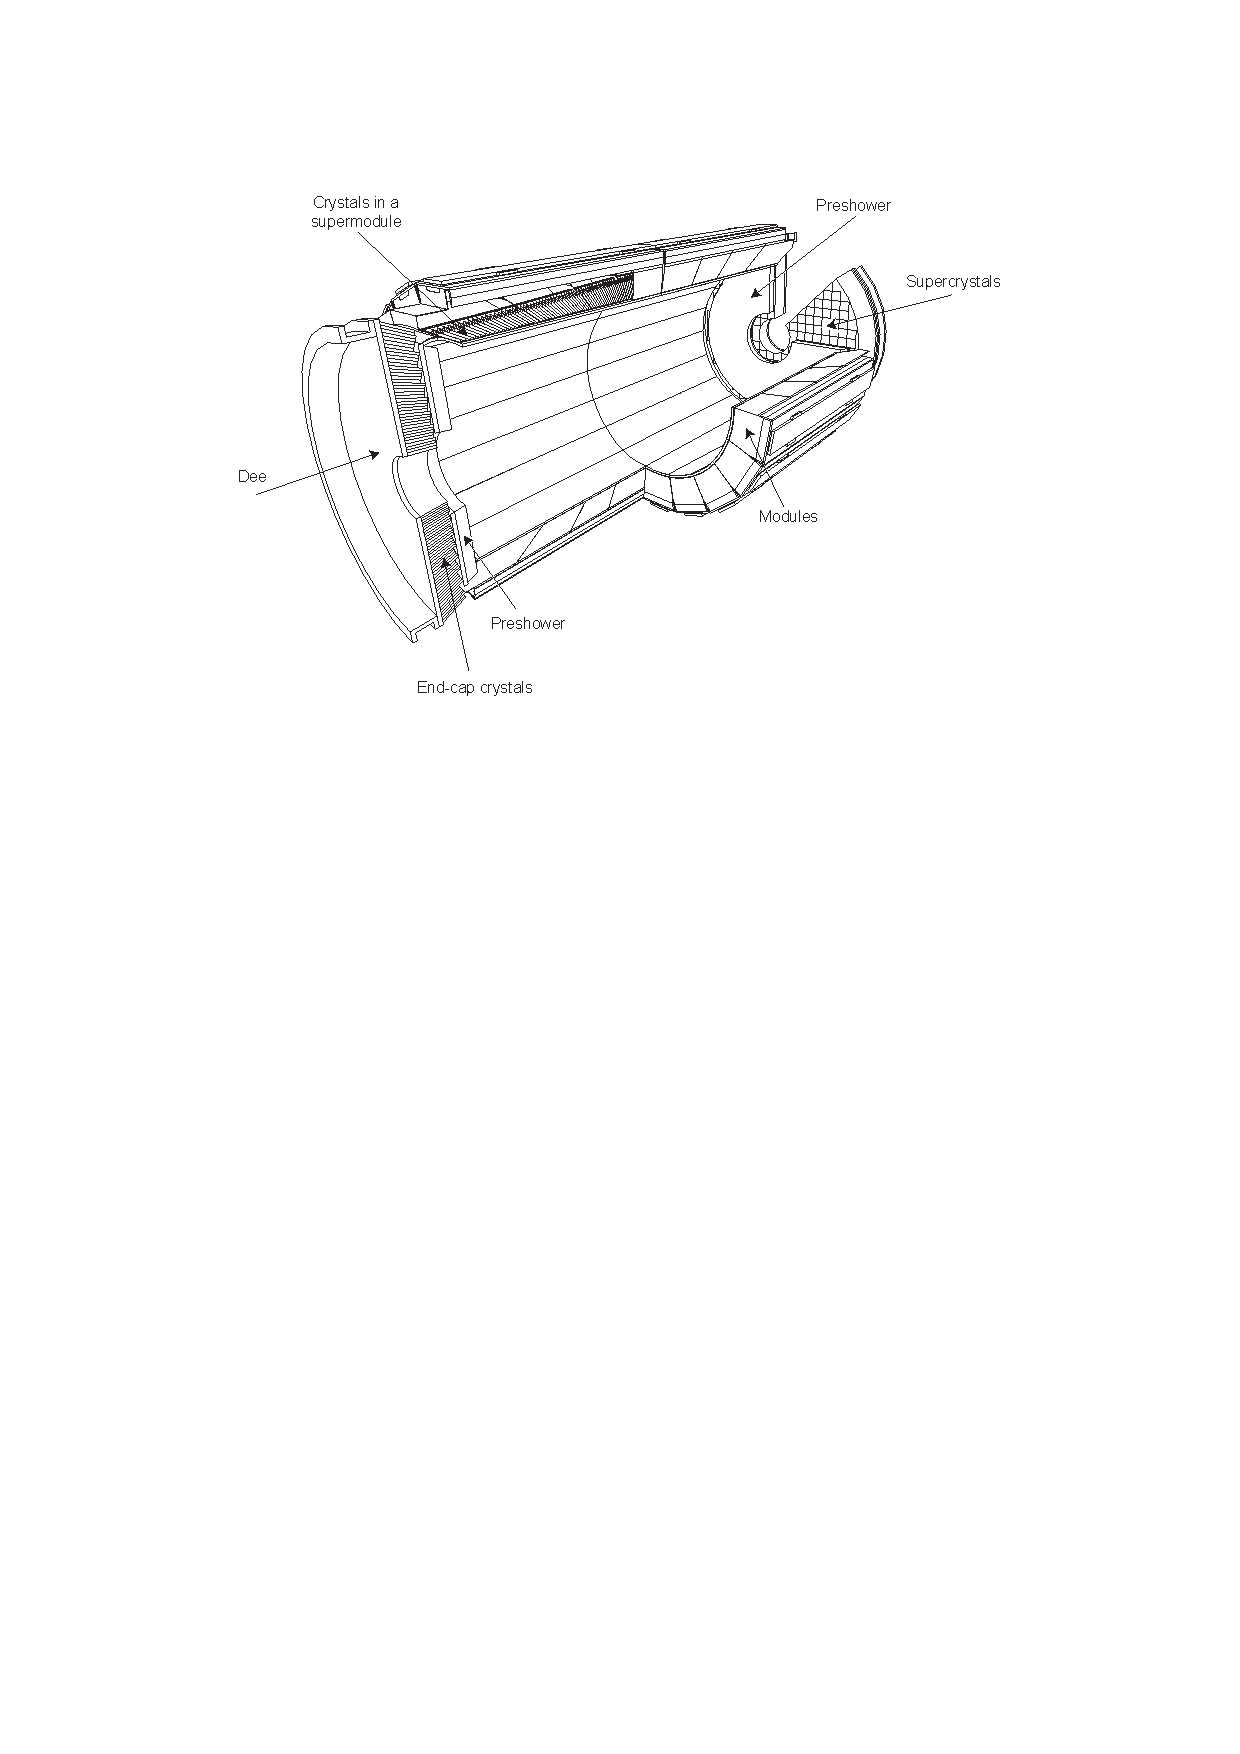
\includegraphics[width=0.9\textwidth]{Detector/Figures/cms_ecal.pdf}
  \caption{
    The layout of the CMS electromagnetic calorimeter.
    The barrel and endcap calorimeters are shown.
    The pre-shower detector sits in front of the endcaps.
    Reprinted from Reference~\cite{}. % https://iopscience.iop.org/article/10.1088/1748-0221/3/08/S08004/meta
  }
  \label{fig:cms_ecal}
\end{figure}

Figure~\ref{fig:cms_ecal} shows the layout of the ECAL.
The central barrel region (EB) has 61200 crystals arranged in a $170\times360$ $\eta$-$\phi$ grid ($0.0174\times0.0174$ granularity) with a coverage up to $\abs\eta = 1.44$ while the two endcap annuli (EE) each have 7324 crystals organized in a $x$-$y$ grid with coverage in the range $1.479 < \abs\eta < 3.0$.
Each crystal in the EB has a truncated pyramidal shape with a length of 230\mm, a $22\mm \times 22\mm$ front-face cross-section, and a $26\mm \times 26\mm$ rear-face cross-section while a crystal in the EE has a cuboid-like shape with a length of 220\mm, a $28.6 \mm \times 28.6\mm$ front-face cross-section, and a $30\mm \times 30\mm$ rear-face cross-section. 
The cross-sectional area of approximately one Moliere radius and length of approximately 25 radiation lengths allows just a few crystals to contain the entire transverse and longitudinal development of the shower.
To reduce the likelihood of the primary photon or electron emerging from the hard scattering depositing most of its energy in passive material, the crystals do not point directly to the interaction region.

The interactions between the 3.8 T magnetic field and the geometries of the ECAL lead to the selection of different photosensors in the barrel and endcaps.
In the endcaps, the magnetic field is parallel to the path of the photoelectrons and has a negligible effect on the gain, while in the barrel, the magnetic field is perpendicular and reduces the gain by a factor proportional to the distance traveled by the photoelectrons.
Thus, in the barrel, solid-state reverse-structure avalanche photodiodes (APDs) with a depletion layer of $6.0\pm0.5\mum$ are used, while photomultiplier tubes with a single gain stage and a very fine copper mesh anode called vacuum phototriodes (VPTs) are used in the endcaps. 
Two APDs with an active area of $25\mm^2$ are glued to the rear of each crystal in the barrel while only one VPT with an active area of $280\mm^2$ is needed per crsytal in the endcap.
The APDs and VPTs amplify the initial signal of approximately 4.5 photoelectrons per \MeV of energy deposit per crystal by a factor of 50 and 10, respectively. 

The small signals from the photodetectors are shaped and amplified in the Multi-Gain Preamplifier (MGPA) and a 12-bit analog-to-digital converter (ADC) samples the pulse every 25\ns.
Each output voltage pulse has a length of approximately 300\ns, with the maximum at approximately 75\ns\ and a slow decay afterwards. 
The MGPA has multiple gain modes of 12, 6, and 1, and the gain chosen for the output decreases once the signal has saturated the previous gain setting.
After the pulse falls below the saturation threshold, the lower gain setting is maintained for the next five samples.
This mechanism provides a dynamic signal range from a few MeV to a maximum of1.5\TeV in the barrel and 3.1\TeV in the endcaps.

The energy resolution of the ECAL was measured using an electron beam to be
\begin{equation}
  \frac{\sigma_E}{E} = \frac{2.8\%}{\sqrt{E/\GeV}} \oplus \frac{12\%}{E/\GeV} \oplus 0.3\%,
\end{equation}
where $E$ is the energy of the incident particle and the three terms on the RHS are the stochastic, noise, and constant terms, respectively.
The stochasistic term is dominated by event-to-event fluctuations in the lateral shower containment and a photostatistics contribution of 2.1\%.
Electronic and digitization noise drive the noise term while the constant term comes from a non-uniform longitudinallight collection and intercalibration errors.

\subsection{Preshower Detector}

At high momenta and high $\abs\eta$, the two photons from a $\pi^0$ decay can merge into a single ECAL crystal due to the large boost in the the $z$-direction of the initial state.
By forcing the initiation of an electromagnetic shower in a region with high spacial resolution in front of the ECAL endcaps, the preshower detector can differentiate between one- and two-photon deposits in the region $1.6 < \abs\eta < 2.5$.
The preshower detector consists of two alternating layers of passive lead absorbers and active silicon strip sensors.
The first (second) lead layer is two (one) radiation lengths thick and the subsequent sensor plane has vertical (horizontal) strips of 6\cm length and 1.9\mm pitch.
The silicon strips resolve the shower with a resolution of $\mathcal{O}(1-10)\mm$, enabling the disambigutation of two nearly collinear photons and the identification of $\pi^0$ decays.

\section{Hadronic Calorimeter}

The hadronic calorimeter (HCAL) is a set of four heterogenous calorimeters that provide hermetic coverage when combined:  the barrel calorimeter (HB) covering $\abs\eta< 1.3$, the endcap calorimeter (HE) covering $1.3 < \abs\eta < 3$, the outer calorimter (HO) covering $\abs\eta < 1.3$, and the forward calorimeter (HF) covering $3 < \abs\eta < 5$.
The region covering $\abs\eta < 3$ shall be referred to as the central HCAL.
The granularity of the HCAL in $\eta$-$\phi$ is $0.087\times0.087$ for $\abs\eta<1.6$, $0.17\times0.17$ for $1.6 < \abs\eta < 3.0$, and $0.175\times0.175$ for $3 < \abs\eta < 5$.
The layout of the HCAL is shown in Figure~\ref{fig:cms_hcal}. 

\begin{figure}[htbp]
  \centering
  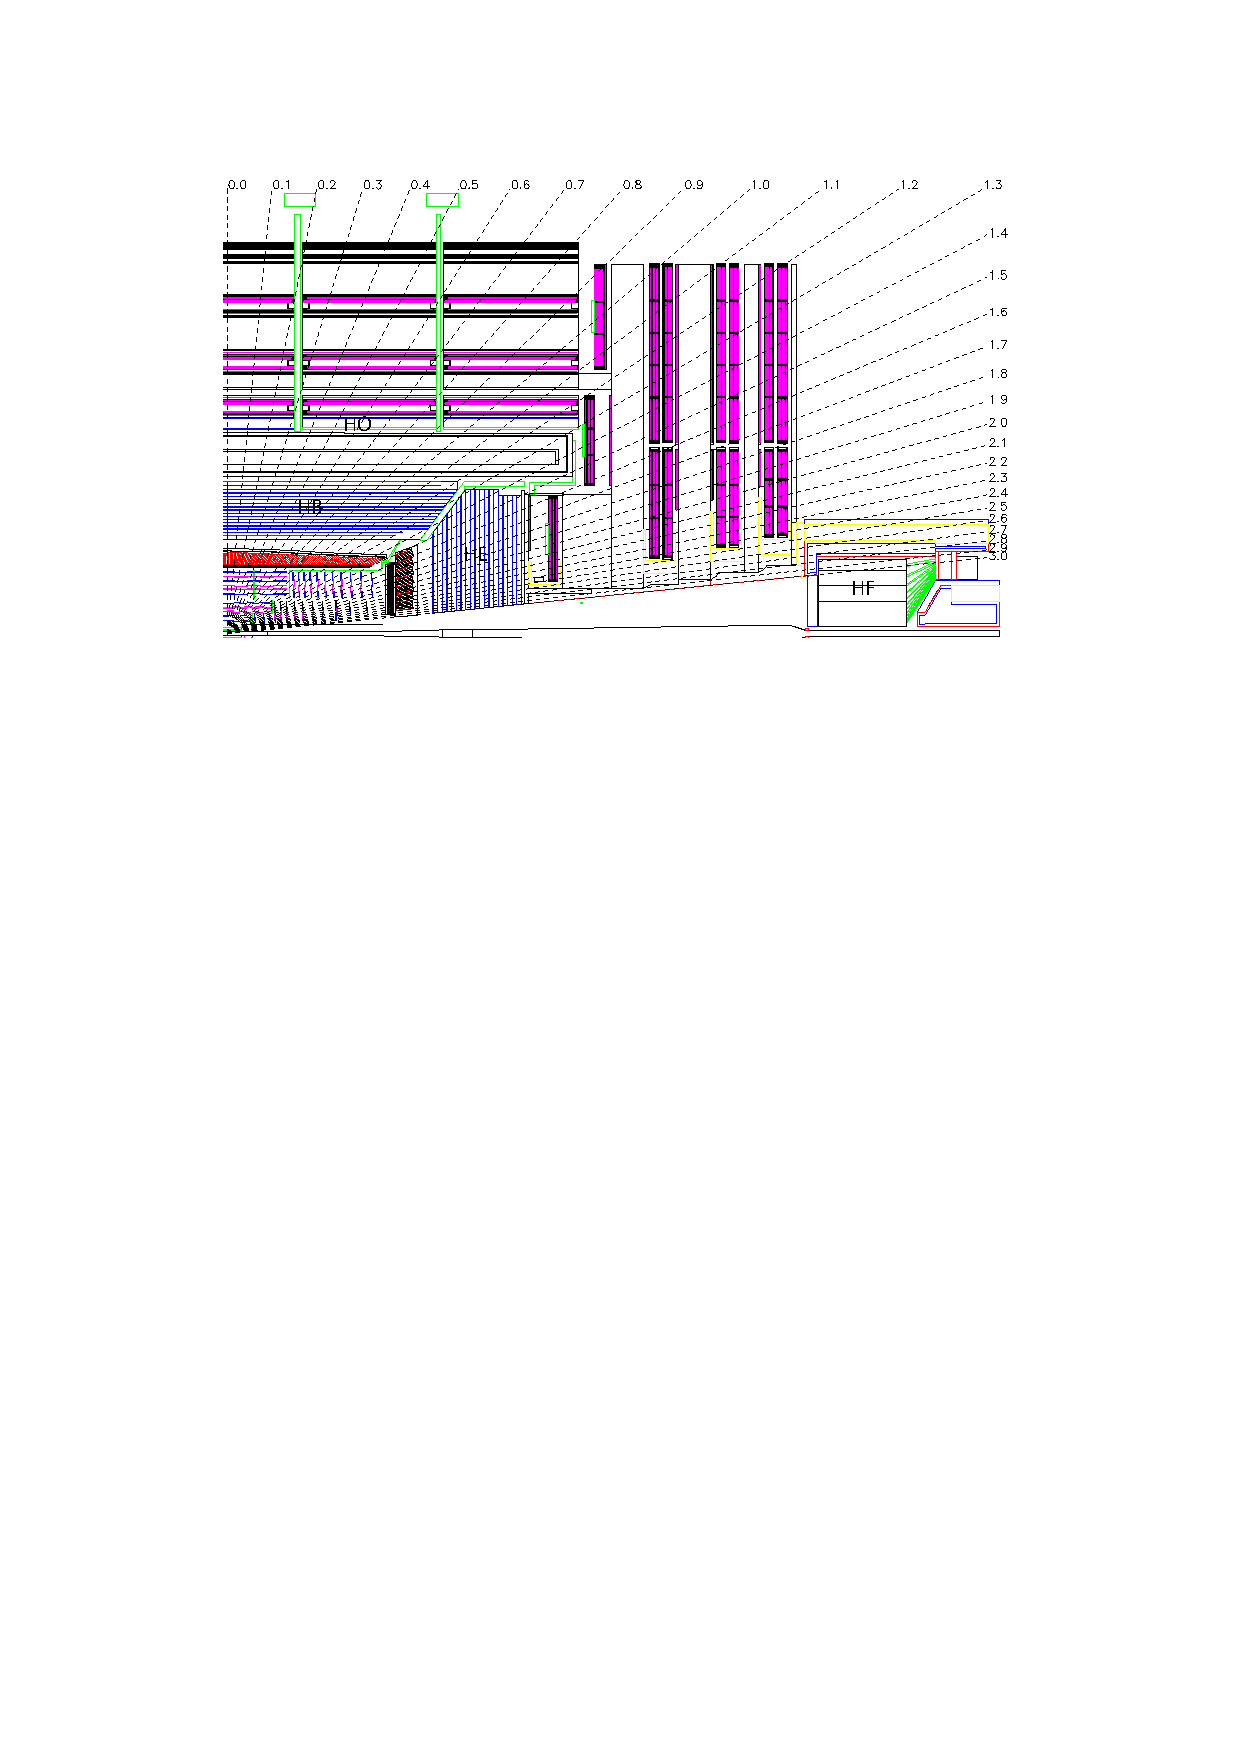
\includegraphics[width=\textwidth]{Detector/Figures/cms_hcal.pdf}
  \caption{
    The layout of the CMS hadronic calorimeter.
    The barrel, endcap, outer, and forward calorimeters are shown and labeled.
    The muon chambers are shown but not labeled. 
    The dashed lines denote different values of pseudorapidity.
    Reprinted from Reference~\cite{}. % https://iopscience.iop.org/article/10.1088/1748-0221/3/08/S08004/meta
  }
  \label{fig:cms_hcal}
\end{figure}

The HB and HE are sampling calorimeters with 16 and 17 thin plastic scintillator layers, respectively,  interleaved with thick absorber layers made of a non-magnetic brass alloy with an interaction length $\lambda_I = 1.5\cm$.
The layers range in thickness from 40 to 75\mm providing a total absorber depth ranging from a minumum of 5.82 $\lambda_I$ at $\abs\eta=0$ to a maximum of 10.6 $\lambda_I$ at $\abs\eta = 1.3$ in the barrel and approximately nine interaction lengths throughout the endcaps, with the ECAL contributing another interaction length worth of material.
The dimensions of the HB and HE are determined by the requirement that they reside between the ECAL and the solenoid. 
To circumvent this constraint, an additional layer of scintillator located in the return yoke of the magnet, the HO, utilizes the solenoid material as an additional interaction length of absorber.
Hybrid photodiodes (HPDs) are used to read out the scintillator light in the HB and HE while silicon photomultipliers (SiPMs) are used in the HO.

Located 11 meters from the interaction point, the HF is a sampling calorimeter covering the region of  phase-space with high pseudorapidity.
Since the particle flux here is much higher than in the central region, the HF uses radiation-hard steel absorber instrumented with two sets of scintillating quartz fibers.
Charged particles produced by showers in the steel traverse the quartz fibers and emit Cherenkov radiation that is recorded by photomultiplier tubes.
To distinguish hadrons from photons and electrons, the second set of fibers starts at a depth of 22\cm.

Since hadrons interact with the ECAL as well as the HCAL, the energy resolution of the detectors must be considered in tandem in the central region.
Using a charged particle test beam, the combined ECAL+HCAL energy resolution was measured to be
\begin{equation}
   \frac{\sigma_E}{E} = \frac{0.847}{\sqrt{E/\GeV}} \oplus 0.074
\end{equation}
and the standalone HF energy energy resolution is
\begin{equation}
   \frac{\sigma_E}{E} = \frac{1.98}{\sqrt{E/\GeV}} \oplus 0.09.
\end{equation}

\section{Muon Chambers}

The outer most components of CMS are the muon triggering, identification, and detection chambers.
These muon detectors are interleaved with the steel return yoke of the magnet resulting in a characteristic $S$-shape for the muon trajectories due to the reversal of magnetic field direction across the solenoid.
Signal purity in the muon detectors is high as hadrons, electrons, and photons are stopped by the calorimeters while muons are minimum ionizing particles (MIPs) that lose little energy while traversing the detector.
Taking advantage of the large detector volumes required by the outer solenoid radius of 3.5\unit{m}, three types of gas ionization chambers are used: drift tubes (DTs) in the barrel covering $\abs\eta < 1.2$, cathode strip chambers (CSCs) in the endcaps coering $0.9 < \abs\eta < 2.4$, and resistive plate chambers (RPCs) in both covering $\abs\eta < 2.1$.
The layout of the muon detectors is shown in Figure~\ref{fig:cms_muons}.

\begin{figure}[htbp]
  \centering
  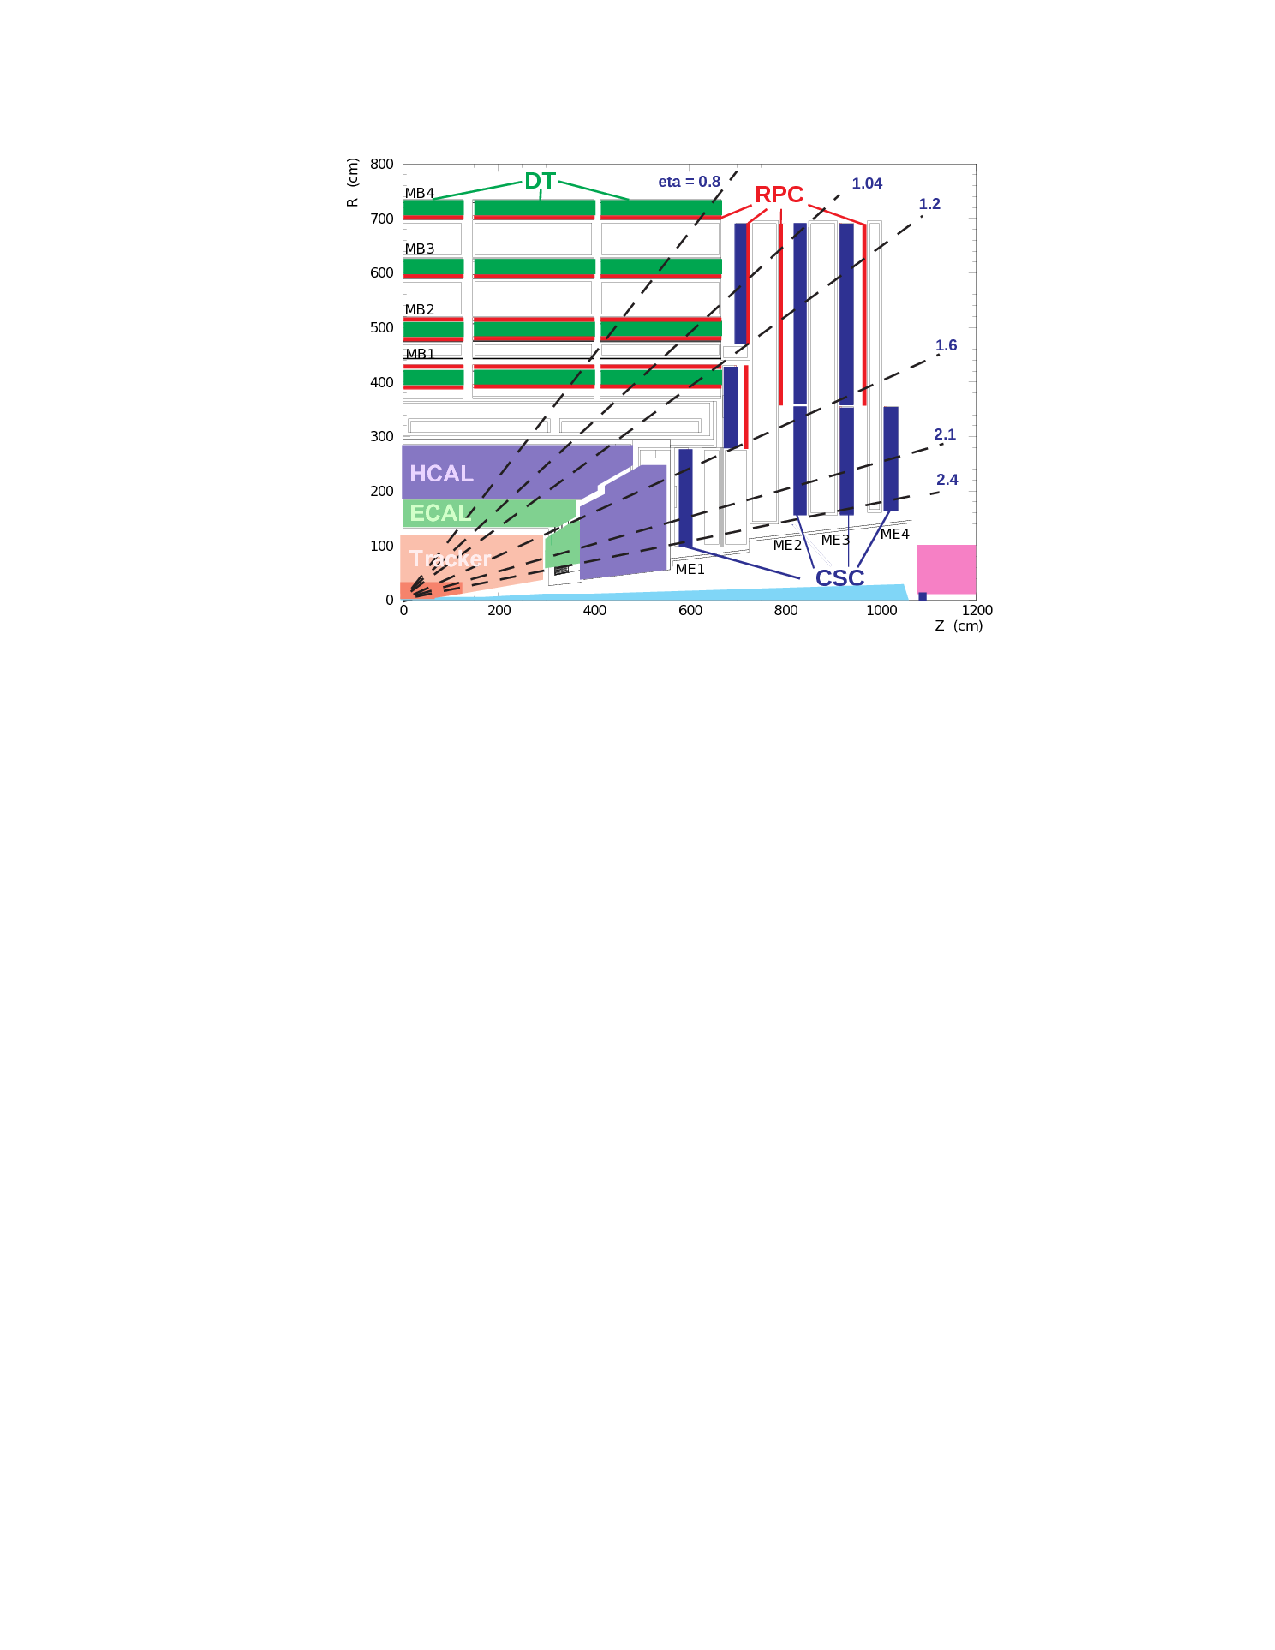
\includegraphics[width=0.9\textwidth]{Detector/Figures/cms_muons.pdf}
  \caption{
    The layout of the CMS muon chambers.
    The four DT stations are labeled MB1-MB4, the four CSC stations are labeled ME1-ME4, and the RPC stations are shown in red.
    The dashed lines denote different values of pseudorapidity.
    Reprinted from Reference~\cite{}. % 
  }
  \label{fig:cms_muons}
\end{figure}

The DT chambers consist of rectangular drift cells with tranverse dimensions of $42\mm \times 13\mm$ filled with a 85:15 Ar/CO$_2$ mix and a gold/steel anode wire held at a voltage of 3.6\unit{kV}.
The  maximum drift time per cell of 400\ns\ provides a spatial resultion of approximately 250\mum.
A single chamber is made out of superlayers which are in turn made out of four individual cells for a combined resultion of 100\mum.
The chambers are arranged into four 2.4\unit{m} thick dodecagonal rings called the muon barrel stations.
All four stations have two superlayers per chamber that measure position in the $r$-$\phi$ plane while the chambers in the inner three stations have an additional superlayer that measures position in the $r$-$z$ plane.
Together, the four muon stations and iron yokes form a wheel with one between the solenoid and the first iron layer, two in between the yokes, and one outside.
The outer barrel is composed of five wheels in total. 

Due to their faster response time and better spatial resolution, CSCs are used to handle the higher muon and background fluxes in the endcap region. 
Each CSC is filled with a 50:40:10 CO$_2$/Ar/CF$_4$ mix and instrumented with 80 cathode strips held at voltages of 2.9-3.6\unit{kV} relative to the gold-plated tungsten anode wires.
The strips run radially outward to measure position in the $r$-$\phi$ plane while the wires run perpendicular measure the $\eta$ and beam-crossing time of the muons.
The four muon stations in each endcap are made of CSCs arranged into annuli oriented perpendicular to the beam axis and interspersed between the flux return plates.
The three inner stations have multiple annuli with smaller ones fitting inside the larger ones while the fourth station only has one close to the beamline.

An RPC is a parallel-plate double-gap chamber with a time resolution of one nanosecond and a poor spatial resolution. 
The RPCs are interspersed throughout the DT and CSCs to provide an independent muon trigger system that can identify the correct bunch crossing time.

\section{Online Trigger System}

To achieve an instantaneous luminosity of $\mathcal{O}(10^{34}) \percms$, the LHC has bunch crossings every 25\ns\ for a total data rate of 40\unit{MHz}, much higher than the 100\unit{kHz} readout rate for the detector and the $\mathcal{O}(1)\unit{kHz}$ data reconstruction and tape writing rates.
Fortunately, uninteresting elastic scattering and QCD inelastic scattering events dominate the approximately 100\unit{$\mu$b} total proton-proton cross-section at the LHC.
Meanwhile, most new physics processes have a predicted on the order of picobarns or femtobarns and even the highest rate SM EWK cross-sections are $\mathcal{O}(10)$\unit{nb}, so not every event needs to be readout, reconstructed, and written to tape.

A two-stage trigger system selects the events to keep for permanent storage and analysis.
The Level 1 hardware-based trigger (L1) selects interesting events based on incomplete detector information to reduce readout and computation times.
Events selected by the L1 trigger are fully readout and passed to the high level software-based trigger (HLT).
The HLT reconstructs the full event on a CPU farm using a version of the offline reconstruction software optimized to process a single event within 200\unit{ms} at the cost of precision.
Events selected by the HLT are sent to the offline computing resources for full reconstruction followed by storage on disk and tape. 

\section{Detector Simulation}

The Geant4 program is used to simulate the detector response to the particles produced in collisions.
Starting with the output of the particle-level MC described in Section~\ref{sec:collider_pheno}, final state particles are propagated through the solenoid's magnetic field into the passive and active elements of the detector where energy deposition, decay, and showering are simulated.
Additional inelastic proton-proton collision are overlaid into an event to simulate the effects of pileup.
As the particles interact with the detector, the response of the readout electronics is simulated, including the effects of noise.
In order to miminize differences between simulated events and those from collisions, the reconstruction software and output format are the same for both up to the retention of additional truth information from the generators.

